\documentclass[a1paper,landscape,25pt]{tikzposter}

\usepackage{amsmath}
\usepackage{amssymb}
\usepackage{tikz}
\usetikzlibrary{calc}

\newcommand{\tikzmark}[2]{\tikz[baseline,anchor=base,remember picture] \node (#1) {#2};}

\usepackage{graphicx}
\usepackage{calc}
\newlength{\depthofsumsign}
\setlength{\depthofsumsign}{\depthof{$\sum$}}
\newlength{\totalheightofsumsign}
\newlength{\heightanddepthofargument}

\newcommand{\nsum}[1][1.4]{% only for \displaystyle
    \mathop{%
        \raisebox
            {-#1\depthofsumsign+1\depthofsumsign}
            {\scalebox
                {#1}
                {$\displaystyle\sum$}%
            }
    }
}
\newcommand{\resum}[1]{%
    \def\s{#1}
    \mathop{
        \mathpalette\resumaux{#1}
    }
}

\newcommand{\resumaux}[2]{% internally
    \sbox0{$#1#2$}
    \sbox1{$#1\sum$}
    \setlength{\heightanddepthofargument}{\wd0+\dp0}
    \setlength{\totalheightofsumsign}{\wd1+\dp1}
    \def\quot{\DivideLengths{\heightanddepthofargument}{\totalheightofsumsign}}
    \nsum[\quot]%
}

% http://tex.stackexchange.com/a/6424/16595
\makeatletter
\newcommand*{\DivideLengths}[2]{%
  \strip@pt\dimexpr\number\numexpr\number\dimexpr#1\relax*65536/\number\dimexpr#2\relax\relax sp\relax
}
\makeatother

\settitle{
  \vspace{-5cm}
  \centering \vbox{
\@titlegraphic \\[\TP@titlegraphictotitledistance] \centering
\color{titlefgcolor} {\bfseries \fontsize{90}{100} \sc \@title \par}
\vspace{2em}
}}

\title{Integralen}

\addtolength{\jot}{1em}

\usetheme{Basic}
\usecolorstyle[colorPalette=PurpleGrayBlue]{Russia}

\tikzposterlatexaffectionproofoff

\begin{document}

\maketitle

\begin{columns}
  \column{0.55}

  \block{Basisregels}{
    \Large
    \begin{align*}
      \int 0\,dx &= C\\
      \int c\,dx &= cx + C\\
      \int x^n\,dx &= \frac{x^{n+1}}{n+1}+C \qquad (n\neq -1)\\
      \int \big(f(x)\pm g(x)\big)\,dx &= \int f(x)\,dx \pm \int g(x)\,dx\\
      \int c\cdot f(x)\,dx &= c\int f(x)\,dx
    \end{align*}
  }

  \block{Veelgebruikte Integralen}{
    \Large
    \begin{align*}
      \int \frac{1}{x}\,dx &= \ln|x|+C \ (x\neq 0) &
      \int \sqrt{x}\,dx &= \frac{2}{3}x^{3/2}+C \ (x\ge 0)\\
      \int e^x\,dx &= e^x + C &
      \int a^x\,dx &= \frac{a^x}{\ln(a)}+C \ (a>0,\ a\neq 1)\\
      \int \sin x\,dx &= -\cos x + C &
      \int \cos x\,dx &= \sin x + C\\
      \int \tan x\,dx &= -\ln|\cos x| + C &
      \int \cot x\,dx &= \ln|\sin x| + C\\
      \int \frac{1}{1+x^2}\,dx &= \arctan x + C &
      \int \frac{1}{\sqrt{1-x^2}}\,dx &= \arcsin x + C \ (|x|<1)
    \end{align*}
  }

  \column{0.45}

  \block{Substitutie en Partiële Integratie}{
    \Large
    \begin{align*}
      \int f\big(g(x)\big)\,g'(x)\,dx &= \int f(u)\,du \quad (u=g(x))\\[0.6em]
      \int f\,dg &\overset{PI}{=} fg-\int g\,df
    \end{align*}
  }

  \block{Definitie en Hoofdstelling}{
    \Large
    \begin{align*}
      \int_a^b f(x)\,dx &= \lim_{n\to\infty}\sum_{i=1}^{n} f(\xi_i)\,\Delta x && \big(\Delta x=\tfrac{b-a}{n},\ \xi_i\in[x_{i-1},x_i]\big)\\
      \int_a^b f(x)\,dx &= F(b)-F(a) && (F'=f)
    \end{align*}
  }

\block{Riemannsom}{
  \LARGE
  \begin{center}
    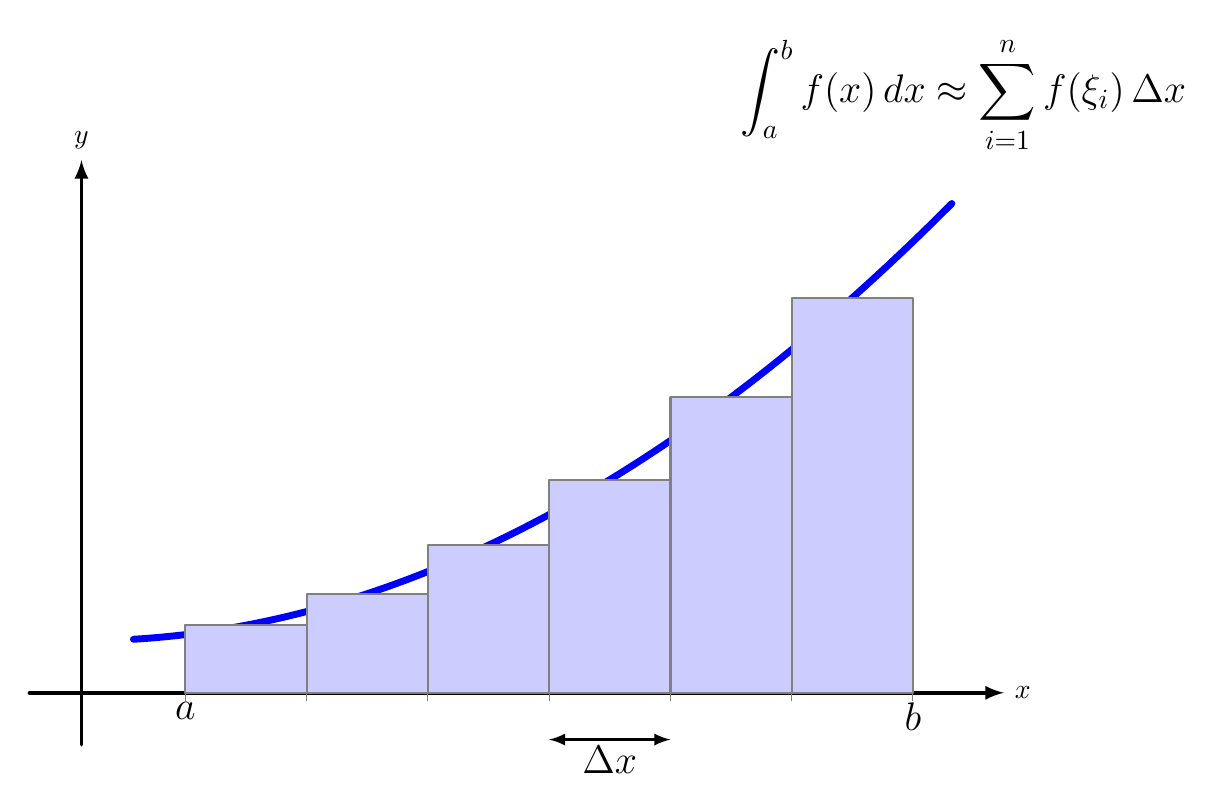
\begin{tikzpicture}[scale=3.3, line cap=round, line join=round, >=latex]
      % Kies een voorbeeldfunctie
      \def\fA{0.15} \def\fB{0.2}
      \def\f(#1){\fA*(#1)*(#1) + \fB}

      % Interval en aantal rechthoeken
      \pgfmathsetmacro{\a}{0.4}
      \pgfmathsetmacro{\b}{3.2}
      \pgfmathsetmacro{\n}{6}
      \pgfmathsetmacro{\dx}{(\b-\a)/\n}

      % Assen
      \draw[->, line width=1.3pt] (-0.2,0) -- (3.55,0) node[right] {$x$};
      \draw[->, line width=1.3pt] (0,-0.2) -- (0,2.05) node[above] {$y$};

      % Functiecurve
      \draw[line width=2.5pt, color=blue, samples=140, domain=0.2:3.35]
        plot (\x, {\f(\x)});

      % Rechthoeken (midpoint rule: \xi_i = midden van [x_{i-1},x_i])
      \foreach \i in {1,...,6}{
        \pgfmathsetmacro{\xL}{\a + (\i-1)*\dx}
        \pgfmathsetmacro{\xR}{\a + \i*\dx}
        \pgfmathsetmacro{\xi}{(\xL+\xR)/2}
        \pgfmathsetmacro{\h}{\f(\xi)}

        % Rechthoek
        \fill[blue!20] (\xL,0) rectangle (\xR,\h);
        \draw[gray, line width=0.8pt] (\xL,0) rectangle (\xR,\h);

        % Partitiepunten op de x-as
        \draw[gray] (\xL,0) -- (\xL,-0.03);
        \ifnum\i=6\relax
          \draw[gray] (\xR,0) -- (\xR,-0.03);
        \fi

        % Een voorbeeld van \xi_i en f(\xi_i) label (alleen bij i=3 om het rustig te houden)
        % \ifnum\i=3\relax
        %   \fill[black] (\xi,\h) circle (1.5pt) node[above left] {$\big(\xi_i,f(\xi_i)\big)$};
        %   \draw[dashed, gray] (\xi,0) -- (\xi,\h);
        % \fi
      }

      % Labels a en b
      \node[below] at (\a,0) {\Large $a$};
      \node[below] at (\b,0) {\Large $b$};

      % Delta x pijl onderaan
      \pgfmathsetmacro{\xLdx}{\a+3*\dx}
      \pgfmathsetmacro{\xRdx}{\a+4*\dx}
      \draw[<->, line width=1pt] (\xLdx,-0.18) -- (\xRdx,-0.18)
        node[midway, below, inner sep=2pt] {\Large $\Delta x$};

      % Formule van de Riemannsom
      \node[anchor=west] at (2.5,2.3) {\Large
        $\displaystyle \int_a^b f(x)\,dx \approx \sum_{i=1}^{n} f(\xi_i)\,\Delta x$
      };
    \end{tikzpicture}
  \end{center}

  \Large
  \begin{center}
    $\xi_i \in [x_{i-1},x_i]$ en $\Delta x = \dfrac{b-a}{n}$.
  \end{center}
}
\end{columns}

\end{document}
